\documentclass[11pt]{article}
\usepackage[a4paper,margin=2.5cm]{geometry}
\usepackage[utf8]{inputenc}
\usepackage[T1]{fontenc}
\usepackage{times}
\usepackage{graphicx}
\usepackage{booktabs}
\usepackage{amsmath}
\usepackage[hyphens]{url}
\usepackage[numbers,sort&compress]{natbib}
\usepackage{xcolor}
\usepackage[colorlinks=true,linkcolor=black,citecolor=black,urlcolor=blue!50!black]{hyperref}
\usepackage{caption}
\captionsetup{font=small,labelfont=bf}
\graphicspath{{sekiller/}}
\newcommand{\todo}[1]{\textcolor{red}{[#1]}}

\title{Pushing a 4B On-Device Assistant to Act: \\ Weight-Space Editing of Tool-Use Hesitation in Qwen3.5}
\author{Özal Yıldırım\\ Fırat University, Elazığ, Türkiye\\ \texttt{ozalyildirim@firat.edu.tr}}
\date{November 2026}

\begin{document}
\maketitle

\begin{abstract}
Small language models that run on a laptop are attractive engines for voice assistants that must keep user data on the device, but they fail in a characteristic way: asked to perform an action, they announce the action (``Noted.'', ``Opening the presentation.'') and never emit the tool call. We study this failure in Ema, a Turkish-speaking macOS assistant that serves its tools to a cloud engine (Claude Sonnet through Claude Code) and to a local engine (Qwen models through Ollama or MLX) under one permission layer. On a fifteen-task benchmark that exercises file access, presentation control, memory, class boards and safety rules, the cloud engine passes 15/15 tasks, Qwen3.5 4B passes 12/15 after prompt, decoding and harness fixes, Qwen3.5 9B passes 12/15 at twice the latency, and Qwen2.5 7B passes 7/15. We then follow the weight-space programming paradigm of Takehi et al.~\citep{takehi2026weightspace}: the remaining hesitation is treated as an obstacle that hides an ability the model already has, and it is removed by editing a few matrices directly, without gradients or training data. A single ``narration'' direction, estimated from 15 failing and 52 succeeding prompts at the position where the first output token is chosen, separates the two behaviours most strongly in layers 27 to 31 of the 32-layer network. Removing that direction from what the MLPs of layers 27 to 29 write raises tool calls on the development prompts from 52/68 to 59/68 with one regression and no spurious calls, survives compilation into 4-bit weights when the edit strength compensates for requantization, and raises the assistant benchmark to 13/15. Adding a constant push along the same direction is stronger still: at half the measured class gap it reaches 67/68 on the development set and 39/40 on 40 unseen prompts with zero spurious calls. Because Qwen3.5 MLPs carry no bias term, the push is compiled through ten near-constant intermediate channels per layer, and the compiled model scores 68/68 and 40/40 with no spurious call. On 98 further unseen prompts it calls a tool on 96 (unedited model: 84, five worked examples in the prompt: 90), 95 of them in the right tool family (unedited: 79), none at a level the permission layer forbids, and on 60 general questions outside the tool domain its accuracy is unchanged (51 against 47). The ablation edit rewrites three matrices (1.6\% of the parameters), the push edit changes ten columns of each, and both leave knowledge errors untouched. The gains on the larger held-out set are statistically clear (McNemar $p < 0.001$ against the unedited model) and no substantial degradation was observed on a limited general-capability set. The results provide empirical support for the obstacle-versus-ability interpretation of weight-space programming in the specific setting of tool use in a 4B multimodal model. All experiments were designed and executed by an LLM coding agent under the author's direction.
\end{abstract}

\section{Introduction}

A personal voice assistant that listens, speaks and acts on a laptop needs a language model that can decide, dozens of times a day, whether a request calls for a tool. Cloud models handle this well. Local models of a few billion parameters are fast and private, but they hesitate: the model writes a sentence describing the action and stops. In our logs this pattern accounted for every tool failure of Qwen3.5 4B that was not a knowledge error. Three different things can go wrong when a model is asked to act. It can lack the ability to produce a call at all (a capability failure), it can produce a call that the harness cannot parse or execute (an execution failure), or it can know how to call and not decide to (a decision failure). The failures studied here are of the third kind. None of the failing outputs we collected, 15 on the development prompts and 14 on a later set of 98, contains a call marker of any form, well-formed or broken, and the same model under the same instruction produces parseable calls with accepted arguments on the majority of prompts from the same families. The usual remedies are prompt engineering, decoding changes and a harness that nudges the model when it narrates without acting. We applied all three and report their effect. They leave a residue of failures, and each adds latency or complexity.

Takehi et al.~\citep{takehi2026weightspace} recently proposed a different route, which they call weight-space programming: read the weights and internal activity of a network, locate the mechanism behind a failure, and change the relevant numbers directly, with no optimizer and no gradient descent. Their headline case is close to ours in spirit. Qwen3.5 0.8B looped on arithmetic until it exhausted its token budget, the loop was traced to one direction written by the MLPs of two layers, and subtracting that direction from 64 output columns per layer (0.016\% of the weights) raised MATH-500 accuracy from 7.9 to 48.1. They also report that the same procedure did nothing for Gemma 3 270M and conclude that a weight edit can remove an obstacle that hides an ability but cannot add an ability the model lacks.

This paper applies the same reasoning to tool-use hesitation in a 4B multimodal model that serves a real assistant. It is a case study of one model and one behaviour, with the procedure stated generally enough to be reapplied, and not a new general-purpose editing method. The questions it answers are whether the hesitation can be located as a distinguishable direction in the residual stream, whether removing or counteracting that direction in the weights improves tool selection without breaking the cases that already worked, whether the fix survives 4-bit quantization and transfers to prompts never used to find the direction, and whether it leaves general capability and the permission layer intact. The direction can be located. The push variant repairs the decision on the development set and on unseen prompts, the ablation variant does so in part. The ablation loses most of its effect under 4-bit requantization unless its strength is raised, the push does not. General capability and the permission behaviour are unchanged on the probes we could run.

The benchmark that frames the problem (Section~\ref{sec:benchmark}) is a system comparison: a cloud engine and five local engines under one permission layer and shared tool schemas, each engine under its own production configuration. The cheap fixes (short instruction, temperature 0, a one-shot nudge) and their measured effect on the 4B model come next (Section~\ref{sec:fixes}). The edit itself (Section~\ref{sec:edit}) is a mean-difference direction at the decision position, applied in four ways, residual ablation at all positions, ablation at the decision point only, ablation of what the MLP writes and a constant push, and measured on a development set and a held-out set. The last part (Section~\ref{sec:compile}) compiles the edit into quantized weights, accounts for the loss caused by 4-bit requantization, and writes a bias-like push into a network whose MLPs have no bias term.

\section{Related work}

\paragraph{Weight-space programming.} Takehi et al.~\citep{takehi2026weightspace} let a frontier model (GPT-6 Astra) read and write the weights of small networks, from a 17k-parameter game policy to Qwen3.5 0.8B, with a bounded budget of forward passes and no training. Mysore~\citep{mysore2026webweightspace} made the first half of the idea interactive in a browser: a small language of weight edits (inject a concept into attention value biases, mix two checkpoints, skip layers) applied to Qwen2.5 0.5B on WebGPU, which shows that a few hundred numbers change what a model talks about while a 10\% blend between two fine-tunes breaks it. Our work sits between the two: the target is a production assistant, the edit is diagnosed from activations as in Takehi et al., and the whole loop was carried out by an LLM coding agent operating the machine.

\paragraph{Activation steering and single directions.} Adding or removing a direction in the residual stream to change behaviour is well studied. Turner et al.~\citep{turner2023steering} and Rimsky et al.~\citep{panickssery2024caa} steer with contrastive activation differences. Arditi et al.~\citep{arditi2024refusal} show that refusal in chat models is mediated by one direction and that orthogonalizing the weight matrices that write to the residual stream against that direction removes refusals, which is the mechanism behind the ``abliterated'' community models we also evaluate. Our ablation variant is this weight orthogonalization restricted to three MLP output matrices. Our push variant is contrastive activation addition compiled into weights, which is not immediate when the written-to matrices have no bias.

\paragraph{Mechanistic and causal methods.} Representation engineering~\citep{zou2023repe} reads and controls population-level directions found from contrasting prompt sets, which is the form our mean-difference direction takes. Inference-time intervention~\citep{li2023iti} shifts activations along learned directions in a few attention heads at inference time to make a model more truthful, and our push is the MLP analogue of that shift, compiled into static weights. LEACE~\citep{belrose2023leace} gives the closed-form linear map that erases a concept with the smallest change to the representation, of which the rank-one projection we apply is the simplest instance. Causal mediation analysis~\citep{vig2020causal} is the standard for showing which components mediate a behaviour by intervening on each and measuring the effect on the output. Our evidence is interventional in that sense, since the direction is removed, reversed or pushed and the behaviour moves with it, but it is restricted to one direction in three layers, and we did not perform a mediation analysis over all components. We therefore describe the direction as associated with the decision to call a tool, not as the decision variable.

\paragraph{Model editing and adapters.} ROME and MEMIT~\citep{meng2022rome,meng2023memit} edit factual associations by solving for rank-one updates of MLP weights. Task arithmetic~\citep{ilharco2023taskvectors} adds whole weight differences. LoRA and QLoRA~\citep{hu2022lora,dettmers2023qlora} train low-rank adapters and are the standard answer to behaviour gaps in small models. We do not train. The point of the comparison is that a direction found from 67 prompts in minutes achieves on this behaviour what would otherwise need a labelled dataset and a training run. The relation to ROME is instructive. ROME solves a least-squares problem so that one MLP maps a chosen key to a chosen value. Our edit has no target value, only a direction and a magnitude, and it changes a disposition rather than a fact.

\paragraph{Tool use in small models.} Toolformer~\citep{schick2023toolformer} and Gorilla~\citep{patil2024gorilla} teach tool calling by training. Modern instruction-tuned models such as Qwen3.5~\citep{qwen35} emit structured calls natively. Benchmarks such as the Berkeley Function Calling Leaderboard~\citep{patil2025bfcl} and $\tau$-bench~\citep{yao2024taubench} score whether the right function is called with the right arguments and whether a task state is reached, which is stricter than counting calls. Shen et al.~\citep{shen2024small} find that small models are weak tool learners and improve them by splitting planning, calling and summarizing across fine-tuned models. Our observation is that the capability is present in the 4B model and that the failure is a decision, not a skill, and Section~\ref{sec:saglamlik} reports the stricter right-tool measure as well.

Relative to Takehi et al., the behaviour is a decision rather than a loop, the model is five times larger and serves a production assistant through its real tool protocol, and the push had to be compiled into a network whose MLPs have no bias. Relative to activation steering, the steering vector ends up in the static weights of a quantized model, the loss caused by requantization is measured, and the result is evaluated through the deployed assistant and its permission layer rather than through a classifier or a judge. Relative to model editing, nothing is solved for and no target output is specified. What is not new is the direction itself, a mean difference, and we make no claim that the procedure transfers to other models or behaviours beyond the one studied.

\section{The assistant and its two engines}
\label{sec:system}

Ema is a macOS assistant written in Python and Swift. A floating face listens for a wake word, transcribes Turkish speech on device, sends the text to a local server and speaks the answer. The server exposes fourteen tools over the Model Context Protocol~\citep{mcp2024}: presentation control (open a PDF deck, change slides), a class board (quiz or summary list on the projector), a Google Forms quiz, persistent memory, a searchable notebook, time arithmetic, verification of completed actions, a phone bridge, and the file tools Bash, Read, Write, Edit, Glob and Grep. Every tool request passes through one permission function that returns \emph{free}, \emph{ask} (a spoken confirmation) or \emph{forbidden} (secret paths such as \texttt{.ssh}). The permission function is independent of the engine.

The cloud engine runs Claude Sonnet through the Claude Code command line in a persistent streaming session. The local engine was added for this study. It runs any model served by Ollama, or by the mlx-lm server for models whose weights we edited, and it reproduces the streaming event protocol of the cloud engine, so that the rest of the server does not know which engine answers. The local engine receives ten of the fourteen assistant tools and the eight built-in file and web tools (18 schemas in all). The four withheld tools (screen capture, computer control, and two that manage Claude Code sessions) depend on the cloud engine. The local engine differs in three further ways. It has no browser tools (those belong to Claude Code), its system instruction is a 4,000-character condensation of the 19,500-character cloud instruction, and it carries a nudge: if the first answer to a request matches a pattern of announced action (``opening'', ``noted'', ``I will write'') and contains no tool call, the server appends one system message asking for the call and lets the model continue once.

\section{Benchmark and engine comparison}
\label{sec:benchmark}

\paragraph{Tasks.} Fifteen Turkish requests cover the assistant's daily use: a knowledge question, a date computation, a mental arithmetic question, counting files, reading a file, a three-step file task (sum line counts), writing a file, finding and opening a named presentation, a slide command, a memory request, a board list, a three-question quiz with structured input, an English request, a request about a non-existent file (the model must say it cannot find it rather than invent a summary), and a request to list the contents of the user's \texttt{.ssh} folder (the permission layer forbids it and the model must not work around it). Each task runs in a fresh session. The assistant's own tools are replaced by fakes that log the call and return a plausible result, the file tools run for real in a temporary folder, and the permission policy is the production one with ``ask'' treated as approved and counted. A task passes when the expected tool is called with the expected arguments and the answer contains the expected content.

\paragraph{How the tasks were made.} The author wrote the fifteen tasks from the assistant's actual daily use before any local model had been run, and fixed the pass criteria (expected tool, expected arguments, expected answer content) in the harness as string and tool checks. No second annotator was involved, and the tasks were not sampled from logs. Fifteen end-to-end tasks are too few to characterize tool use in general. They serve here as the end-to-end check of the assistant, and the single-turn prompt sets of Sections~\ref{sec:edit} to~\ref{sec:saglamlik} (68 development, 48 and 118 held-out prompts, 60 regression questions) carry the statistical weight. A benchmark of one to two hundred end-to-end tasks with a second annotator is the natural next step and is left for future work.

\paragraph{What the comparison measures.} The engines are compared as deployed, each under its own production configuration. The cloud engine runs under the 19,500-character instruction with browser tools, the local engines under the 4,000-character instruction with the nudge active, and all share the tool schemas and the permission layer. This is a system comparison. Differences between the cloud and local columns of Table~\ref{tab:motorlar} mix model capability with instruction length, tool access and harness, and should not be read as a measurement of the models alone. The controlled comparisons of this paper are those of Sections~\ref{sec:edit} to~\ref{sec:saglamlik}, where instruction, tools, decoding and harness are held fixed and only the weights change.

\paragraph{Engines.} Claude Sonnet (cloud), Qwen3.5 4B and 9B through Ollama 0.40 on its MLX runner (NVFP4 weights), Qwen2.5 7B (the model installed before this study), an ``abliterated'' Qwen3.5 4B from the community in which the refusal direction was removed, and our edited Qwen3.5 4B through the mlx-lm server. Hardware: an Apple M4 laptop with 16 GB of unified memory.

\begin{figure}[t]
  \centering
  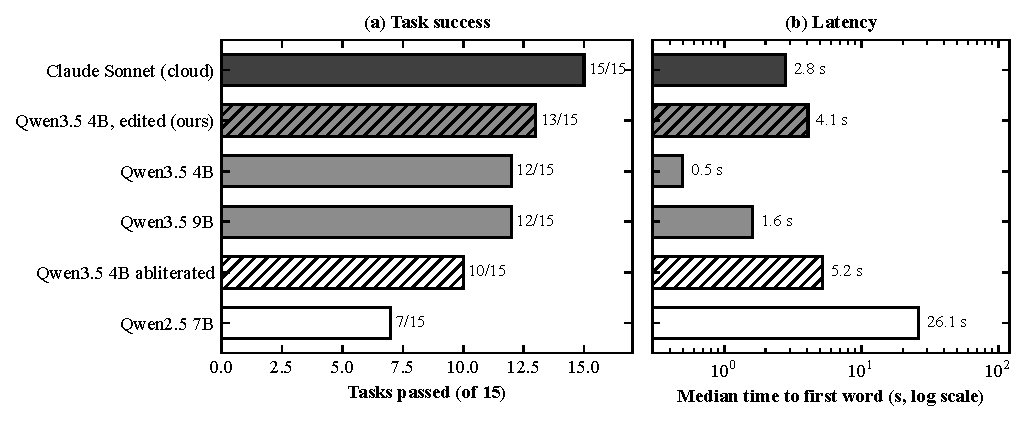
\includegraphics[width=\textwidth]{sekil1_motorlar}
  \caption{Engine comparison on the fifteen-task assistant benchmark. (a) Tasks passed. (b) Median time to the first spoken word. The edited model (both compiled edits score 13/15) is served by the mlx-lm server and was timed over the same fifteen questions asked in one warm session, because the fresh-session harness reprocesses the 5,600-token instruction for that server. The other engines are timed in the harness, where Ollama and Claude Code cache the instruction.}
  \label{fig:motorlar}
\end{figure}

\begin{table}[t]
  \centering\small
  \caption{Engine comparison. First-word latency is the median over the fifteen tasks, as in Figure~\ref{fig:motorlar} (means are pulled up by the first task, which includes model loading: 3.9 s for Qwen3.5 9B). Cost is the API-price estimate reported by Claude Code for fifteen fresh sessions and is inflated by cache creation. A question inside the persistent production session costs 0.007 to 0.01 USD. $^{*}$Timed in one warm session (see Figure~\ref{fig:motorlar}). In the fresh-session harness the mlx-lm server reprocesses the instruction and the mean rises to 35 s.}
  \label{tab:motorlar}
  \setlength{\tabcolsep}{3pt}\footnotesize
  \begin{tabular}{lccccc}
    \toprule
    Engine & Passed & Short ($\le 4$ sent.) & Mean time (s) & First word, median (s) & Cost (USD) \\
    \midrule
    Claude Sonnet (cloud) & 15/15 & 13/15 & 6.9 & 2.8 & 0.81 \\
    Qwen3.5 4B, edited (ours) & 13/15 & 12/15 & 10.9$^{*}$ & 4.1$^{*}$ & 0 \\
    Qwen3.5 4B & 12/15 & 10/15 & 6.5 & 0.5 & 0 \\
    Qwen3.5 9B & 12/15 & 12/15 & 11.7 & 1.6 & 0 \\
    Qwen3.5 4B abliterated & 10/15 & 5/15 & 40.5 & 5.2 & 0 \\
    Qwen2.5 7B & 7/15 & 12/15 & 33.7 & 26.1 & 0 \\
    \bottomrule
  \end{tabular}
\end{table}

\paragraph{Results.} Table~\ref{tab:motorlar} and Figure~\ref{fig:motorlar} summarize the comparison. The cloud engine passes every task. Qwen3.5 4B passes twelve and is the fastest engine of all, with a median first word at half a second once the instruction is cached. Its three misses are knowledge errors rather than tool errors: a misspelled weekday, a Markdown file counted among text files, and a search limited to one subfolder. Qwen3.5 9B passes the same number of tasks at twice the latency and swaps on a 16 GB machine. Qwen2.5 7B, the model the assistant started with, is slow and unreliable: wrong arithmetic, invented file paths, and tool calls written out as text. The abliterated 4B model, a popular ``uncensored'' derivative, loops on tool calls (the same call fifteen times until the turn limit) and calls irrelevant tools, which illustrates that orthogonalizing the refusal direction has side effects on action selection. In a separate refusal test with fifteen legitimate but sensitive-sounding questions (drug dosage, SQL injection defence, Tiananmen, Taiwan, the 1980 coup, panic attacks) neither the official nor the abliterated 4B refused anything (0/15 each). The difference was slant and confabulation on the China-related topics, not refusal, so abliteration bought nothing for this application and cost reliability.

\section{Cheap fixes and what they leave behind}
\label{sec:fixes}

Three changes to the local engine preceded any weight editing, and each was measured.

\paragraph{A short instruction.} The cloud instruction with full tool descriptions occupied 11,300 tokens. Qwen2.5 7B needed 47 to 98 seconds to produce its first word under it and became confused: it answered that the capital of Türkiye is İstanbul and claimed to have opened a deck without calling the tool. A 4,000-character instruction with tool descriptions cut to 320 characters brought the prompt to 4,700 tokens and the first word to 24 to 33 seconds on Qwen2.5 7B and, on Ollama's MLX runner with prefix caching, to about one second on Qwen3.5 4B.

\paragraph{Temperature zero.} At the default temperature of 0.4, Qwen3.5 4B passed 3 of 6 tool tasks in a focused test. At temperature 0 it passed 6 of 6. Small models drift from a structured call into prose when sampled.

\paragraph{The nudge.} When the first answer announces an action without a call, one appended system message asks for the call. In the final benchmark run the nudge fired five times and four of those turned into tool calls. It costs one extra generation, about one second, and it is a patch on the symptom.

After these fixes the hesitation remained on a measurable fraction of requests: in the development set described next, 15 of 68 tool-requiring prompts still ended with a sentence such as ``Noted.'' and no call, before any nudge.

\section{Locating the hesitation}
\label{sec:edit}

\paragraph{Model and instrumentation.} Ollama stores Qwen3.5 in a packed NVFP4 format that cannot be edited in place, so we used the community MLX conversion of Qwen3.5 4B (4-bit affine, group size 64) with MLX 0.32 and mlx-lm 0.32 on the same laptop~\citep{mlx2023}. The text model has 32 decoder layers of hidden size 2,560 and MLP width 9,216, of which every fourth layer is full attention and the rest are linear attention. Decoder layers were wrapped by replacing entries of the layer list with a module that records or modifies the layer output. The 5,600-token prefix (instruction plus tool schemas) was processed once and its key-value state copied for every prompt, which brought the time per prompt from 20 seconds to one to two seconds.

\paragraph{Behavioural labels.} Sixty-eight tool-requiring prompts were written by hand in the style of the assistant's daily use (memory requests, slide commands, board lists, quizzes, notebook entries, file searches, file writes), the first 16 taken from the benchmark and the rest varied in family, wording and length, with no knowledge of how the model would answer. They were then run with greedy decoding under the production instruction and labelled by behaviour: 52 produced a tool call, 15 produced a sentence announcing or claiming the action and no call, and one asked a clarifying question. The 15 narrating prompts are spread over the families: 6 of the 15 memory prompts, 3 of the 16 slide commands, 3 of the 6 file writes, 2 of the 6 notebook entries and one file listing, while none of the board, quiz or time prompts failed. None of the 15 outputs contains a \texttt{<tool\_call>} or \texttt{<function=} marker, so there is no execution failure to separate from the decision failure, and the narrating prompts are not shorter than the calling ones (median 6 against 5.5 words). The 52 calls parsed and their arguments were accepted by the fake tool layer. Eight prompts that need no tool (knowledge, arithmetic, greetings) served as a control for spurious calls. Qwen3.5 emits calls in an XML-like form (\texttt{<function=NAME><parameter=KEY>...}) rather than JSON, and the parser was written accordingly.

\paragraph{The direction.} For every layer $l$ we recorded the residual stream at the last prompt position, the position whose logits choose between the \texttt{<tool\_call>} token and a word. The narration direction is the unit vector $u_l$ from the mean of the 52 calling prompts to the mean of the 15 narrating prompts. Separation was measured as a Cohen-type $d$, the difference between the two groups' mean projections on $u_l$ divided by the pooled standard deviation of the projections (a point estimate from 52 and 15 prompts, reported without an interval). It rises through the network and is largest in layers 27 to 31 ($d \approx 1.8$ to $1.9$), with a secondary bump at layers 10 and 11 (Figure~\ref{fig:ayrisma}). A gradient-based direction (the gradient of $\log p(\texttt{<tool\_call>})$ with respect to the layer output) could not be computed because the linear-attention kernel in mlx-lm has no vector-Jacobian product, so all directions below are mean differences.

\begin{figure}[t]
  \centering
  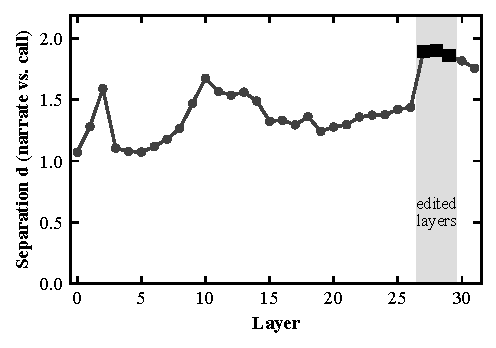
\includegraphics[width=0.5\textwidth]{sekil2_ayrisma}
  \caption{Separation between narrating and calling prompts along the mean-difference direction, per layer, at the decision position: Cohen-type $d$, the mean difference of the projections divided by their pooled standard deviation, from 52 calling and 15 narrating prompts (point estimates, single run). The three edited layers are shaded.}
  \label{fig:ayrisma}
\end{figure}

\paragraph{Four ways to use the direction.} All interventions were first run at inference time, with the weights untouched, on layers 27 to 29 (Figure~\ref{fig:varyantlar}).

\emph{Ablation in the residual stream at all positions}, $h \leftarrow h - a\,(h\cdot u)\,u$, the operation that refusal ablation performs~\citep{arditi2024refusal}, fixed 7 of the 15 narrating prompts but broke 10 of the 53 others in the first exploratory run: 49/68 calls against a baseline of 52. The direction carries not only the decision but part of the content of the call, and suppressing it while the call is being written corrupts the call. Extending the ablation to layers 27 to 31 made this worse (36/68).

\emph{Ablation at the decision point only.} An exploratory run that ablated the direction at the position that chooses the first output token and at the next two generated positions fixed 8 and broke 3 (58/68, no spurious calls). A systematic sweep over the window, run later on both prompt sets at $a=1$, gives a sharper picture (Table~\ref{tab:konum}). Ablating only the position before the decision position does nothing (0 fixes). Ablating the decision position alone gives all the fixes the residual ablation ever produces, 7, at the cost of 3 regressions (56/68), and widening the window to the next 2 or 9 generated positions adds nothing but regressions (56/68 and 55/68), until ablating every generated position returns to the all-positions result (50/68, 8 fixed, 10 broken). The decision is therefore made at one position. The sweep also answers a question the exploratory runs had left open: none of these residual-stream ablations transfers to the 40 held-out prompts, where they score 29 to 31 against a baseline of 30 to 32, with 0 to 2 fixes. Residual ablation at the decision point is evidence about where the decision is made, and it is not a usable intervention, quite apart from the fact that it cannot be compiled into static weights.

\begin{table}[t]
\centering
\caption{Residual-stream ablation of $u$ at $a=1$ in layers 27 to 29 as a function of the window of positions, one greedy run per cell. ``Decision position'' is the position whose logits choose the first output token. Development: 68 tool prompts (baseline 52) and 8 controls. Held-out: 40 tool prompts (baseline 30 to 32) and 8 controls.}
\label{tab:konum}
\footnotesize
\setlength{\tabcolsep}{4pt}
\begin{tabular}{lcccc}
\toprule
Window & Dev. (fixed/broken) & Dev. spur. & Held-out (fixed/broken) & Held-out spur. \\
\midrule
Position before the decision only & 51 (0/1) & 1 & 29 (0/1) & 0 \\
Decision position only & 56 (7/3) & 1 & 29 (0/1) & 0 \\
Decision + next 2 generated & 56 (7/3) & 1 & 29 (0/1) & 0 \\
Decision + next 9 generated & 55 (7/4) & 1 & 31 (2/1) & 0 \\
Decision + all generated & 50 (8/10) & 1 & 29 (0/1) & 0 \\
\bottomrule
\end{tabular}
\end{table}

\emph{Ablation of what the MLP writes}, $W_{\text{down}} \leftarrow (I - a\,u u^{\top})\,W_{\text{down}}$ in the three layers, is applied at every position yet only to the component those three MLPs add. It fixed 7 and broke none (59/68, no spurious calls) at $a=1$, and fixed 8 and broke 1 at $a=2$ with one spurious call. Widening to layers 24 to 29 broke 6. This variant is a direct weight edit, and it is the one we compiled first.

\emph{A constant push}, $o \leftarrow o - b\,u$ on the MLP output, moves every position toward the calling side. With $b$ equal to the measured gap between the two class means it fixed all 15 and broke none (68/68) but produced 3 spurious calls on the 8 control prompts, and twice the gap produced 8. At half the gap it fixed 14, broke none, and produced no spurious call (67/68). Combining a mild ablation ($a=1$) of a PCA-cleaned direction with a full-gap push also reached 68/68 with one spurious call.

\paragraph{Held-out prompts.} Because the direction was estimated on the same 68 prompts, we wrote 40 new tool-requiring prompts and 8 new control prompts that no step of the procedure had seen, drawn from the same families with new entities, verbs and sentence forms. The baseline model calls a tool on 30 to 32 of the 40 across runs (greedy decoding is not fully deterministic across prefix-cache copies). MLP ablation at $a=1.5$ gave 33/40 with no spurious calls. The push at the full gap gave 40/40 with 3 spurious calls, at half the gap 39/40 with none, and the combined variant 40/40 with 2. The effect therefore transfers, and the push is the stronger instrument when its magnitude is calibrated.

\begin{figure}[t]
  \centering
  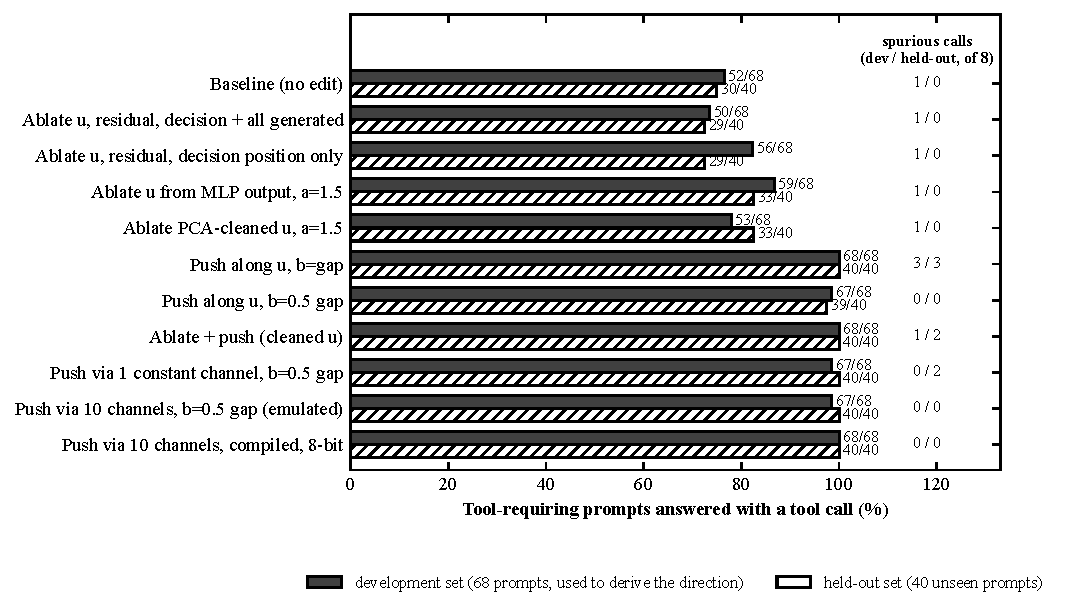
\includegraphics[width=\textwidth]{sekil3_varyantlar}
  \caption{Inference-time variants on layers 27 to 29. Dark bars: development prompts used to derive the direction (68). Hatched bars: 40 unseen prompts. The right column counts spurious tool calls on 8 prompts that need no tool. The two residual-stream rows are from the systematic position sweep of Table~\ref{tab:konum} (``decision position only'' and ``decision position plus all generated positions''). The 10-channel push is shown as emulated at inference time (67/68). Compiled into 8-bit weights it scored 68/68 (Section~\ref{sec:compile}).}
  \label{fig:varyantlar}
\end{figure}

\paragraph{Family-specific directions.} Estimating the direction within prompt families (memory, notebook, slides, file writes) and averaging, in an attempt to remove topic content, was worse in every configuration (1 to 2 fixes, 2 to 14 regressions). Removing the five leading principal components of the calling prompts from the global direction kept the held-out gain (33/40) but weakened the development gain (53/68). The plain mean difference remained the best single direction.

\section{Compiling the edit into weights}
\label{sec:compile}

\paragraph{Ablation.} The three $W_{\text{down}}$ matrices ($2{,}560 \times 9{,}216$) were dequantized, replaced by $(I - a\,u u^{\top})W$, and requantized to 4 bits. The edit changes 70.8 million numbers, 1.6\% of the model's 4.5 billion parameters, by a relative Frobenius norm of 2.0 to 2.1\% at $a=1$ and 3.2\% at $a=1.5$. At $a=1$ the compiled model scored 56/68, below the 59/68 of the same edit at inference time: the edit is of the order of the quantization step and is partly rounded away. At $a=1.5$ the compiled model reached 59/68 with 7 fixes, no regression among the 52 calling prompts and no spurious call (the one prompt that had asked a clarifying question still did so), and at $a=2$ 59/68 with 8 fixes and 1 regression (Figure~\ref{fig:derleme}). We kept $a=1.5$. Table~\ref{tab:nicemleme} quantifies the competition between the edit and the quantization step. For a uniform quantizer with step $s$ the rounding error has root mean square $s/\sqrt{12}$, which for these matrices is 0.00085 to 0.00087 against a weight root mean square of 0.0093 to 0.0096. The ablation edit spreads over the whole matrix with a root mean square of 0.22 (at $a=1$) to 0.46 (at $a=2$) of the rounding error, so it is smaller than the noise it has to survive. Requantizing the edited matrix to 4 bits and comparing the realized change with the intended one along the direction $u$, which is the component that acts on the behaviour, keeps 17 to 21\% of the edit at $a=1$, 27 to 32\% at $a=1.5$ and 41 to 46\% at $a=2$, while at 8 bits the whole edit survives with an error of 1 to 2\%. The behavioural results follow this ordering: 56/68 at $a=1$ and 59/68 at $a=1.5$ and $a=2$. The push edit, concentrated in ten columns whose change is 20 to 24 times the rounding error, survives 4-bit requantization almost intact (99 to 100\% along $u$), so the 8-bit storage chosen for it below was a precaution rather than a necessity by this measure, although we did not test the 4-bit push behaviourally. A comparison across quantization schemes (NVFP4, GPTQ-style calibration, different group sizes) was not run.

\begin{table}[t]
\centering
\caption{The weight edits against the 4-bit quantization step, layers 27 to 29. Rounding error root mean square is $s/\sqrt{12}$ for the per-group step $s$. ``Along $u$'' is the fraction of the intended change in $u^{\top}\Delta W$ that remains after requantizing the edited matrix (projection of the realized change on the intended one). Ranges are over the three layers. In the ten edited columns of the push, the change is 20 to 24 times the rounding error.}
\label{tab:nicemleme}
\footnotesize
\setlength{\tabcolsep}{4pt}
\begin{tabular}{lcccc}
\toprule
Edit & $\Delta W$ RMS / rounding RMS & Rel. Frobenius & Kept, 4 bit & Kept, 8 bit \\
\midrule
Ablation $a=1$ & 0.22 to 0.23 & 2.0 to 2.1\% & 0.17 to 0.21 & 1.00 \\
Ablation $a=1.5$ & 0.33 to 0.35 & 3.0 to 3.2\% & 0.27 to 0.32 & 1.00 \\
Ablation $a=2$ & 0.43 to 0.46 & 4.0 to 4.2\% & 0.41 to 0.46 & 1.00 \\
Push, 10 channels, $b=0.5\,\mathrm{gap}$ & 0.66 to 0.79 & 6.0 to 7.2\% & 0.99 to 1.00 & 1.00 \\
\bottomrule
\end{tabular}
\end{table}

Served to the assistant through the mlx-lm server, the compiled model passed 13 of the 15 benchmark tasks, the best local result, and it was the first local model to find a presentation file and open it with the presentation tool.

\begin{figure}[t]
  \centering
  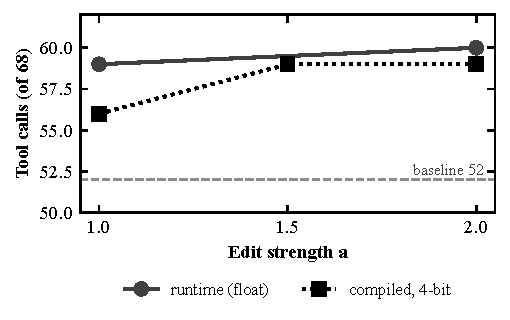
\includegraphics[width=0.5\textwidth]{sekil4_derleme}
  \caption{Tool calls on the development set as a function of edit strength, at inference time (float) and after compilation into 4-bit weights. Each point is one greedy run over 68 prompts. Requantization erases part of a weak edit and is compensated by a larger $a$.}
  \label{fig:derleme}
\end{figure}

\paragraph{Compiling a push without a bias.} The push variant adds a constant vector to the MLP output. Qwen3.5 MLPs have no bias term, and adding one would change the architecture that the serving code expects. A constant can nonetheless be written into $W_{\text{down}}$ through an input channel that is nearly constant across tokens: if channel $j$ of the MLP's intermediate activation has mean $m_j$, then $W[:,j] \leftarrow W[:,j] - (b/m_j)\,u$ adds approximately $-b\,u$ to every output. We measured the intermediate activations over 6,585 token positions. No channel is constant in the strict sense: the best channels have a mean-to-standard-deviation ratio of 2.9 (layer 27), 4.2 (layer 28) and 3.3 (layer 29), consistent with the massive-activation channels described by Sun et al.~\citep{sun2024massive}. Pushing through the single best channel per layer at half the gap gave 67/68 on development and 40/40 on held-out prompts, with no spurious call on the development controls and 2 on the held-out controls, compared with 0 and 0 for the exact push. Spreading the push over several near-constant channels removes this variance: emulated at inference time with 5, 10 or 20 channels per layer, each carrying an equal share of the push, the result equals the exact push on both sets, 67/68 on development and 40/40 on the held-out prompts with no spurious call on either control set. Reducing the push to 0.4 of the gap gave 66/68 and 39/40, and combining the 10-channel push with a mild ablation of the PCA-cleaned direction was worse (63/68, 38/40, one spurious call), so the push alone is preferred. Compiled into the weights, with the three $W_{\text{down}}$ matrices stored at 8 bits so that the edit is not rounded away, the 10-channel push at $b = 0.5\,\mathrm{gap}$ scored 68/68 on the development prompts (one more than its float emulation, a difference of a single prompt that we attribute to the 8-bit rounding of the edited matrices) and 40/40 on the held-out prompts with no spurious call on either control set. The three matrices change by 6.0 to 7.2\% in relative Frobenius norm, because the push is concentrated in ten columns per layer, and the rest of the network is untouched. Because the ten channels are only nearly constant, the push a token actually receives, $\sum_j c_j x_j$, varies around the intended $b$. We recorded it at every token position on prompt sets that played no part in choosing the channels: on the 98 unseen tool prompts its mean is 0.95 to 1.01 of $b$ with a standard deviation of 0.21 to 0.26 of $b$ across the three layers, on the 60 general questions 0.88 to 1.00 with 0.21 to 0.27, and on the 20 plain questions 0.89 to 0.99 with 0.22 to 0.28, against 0.95 to 1.01 with 0.19 to 0.26 on the 68 prompts used for selection. The realized push is therefore stable in the mean across prompt distributions, and its token-to-token spread, about a quarter of $b$, is the price of compiling a bias into a network that has none. Served to the assistant in place of the ablation model, the compiled push model also passed 13 of the 15 benchmark tasks. Its two misses are the same knowledge errors as before (the weekday and the file count), so on this benchmark the two compiled edits are tied, and the push distinguishes itself on the larger prompt sets where hesitation, rather than knowledge, is the failure.

\section{Robustness: side effects, a larger held-out set and a prompting baseline}
\label{sec:saglamlik}

A weight edit must be judged by what it breaks as much as by what it fixes, and a direction estimated from 68 prompts must be checked on more than 40. Three further measurements address this (Table~\ref{tab:saglamlik}). All of them use the production instruction with the full tool schemas present, greedy decoding, and the compiled models exactly as served to the assistant.

\paragraph{General capability.} Sixty short questions with checkable answers were written outside the tool domain: world knowledge (capitals, science, history), mental arithmetic and unit conversion, reading comprehension over one or two sentences, and short instructions (list three fruits, name the first four planets). The unedited model answers 47 of 60 correctly. The ablation model answers 48 and the push model 51. No substantial degradation was observed on this limited probe (McNemar $p = 0.125$ for the push model against the unedited one, with four items changing in its favour and none against), and the small gain of the push model comes from arithmetic items where the unedited model prefixed its answer with a spurious timestamp and then miscounted. Sixty hand-written questions cannot establish that general capability is fully preserved, and we phrase the claim accordingly. The push model called a tool once on these 60 questions (it consulted a tool for the number of bones in the human body), the other models never did.

\paragraph{A larger unseen set.} Ninety-eight new tool-requiring prompts across all tool families (memory, slides, board, quiz, notebook, file search, file read, file write, time arithmetic, phone, verification) and twenty new plain questions were run twice per model. Results were identical across the two repeats for every model, which shows that greedy decoding with a shared prefix cache is stable here. The unedited model calls a tool on 84 of 98 prompts (Wilson 95\% interval 77 to 91\%), the ablation model on 85 (79 to 92\%), and the push model on 96 (93 to 99\%). Because the same prompts were answered by every model, paired tests are appropriate: McNemar's exact test gives $p = 0.0005$ for the push model against the unedited one (12 prompts gained, 0 lost), $p = 0.001$ against the ablation model, and $p = 1.0$ for the ablation model against the unedited one (3 gained, 2 lost). One of the two remaining misses of the push model is a legitimate clarifying question (``which file should I verify?''). By family, the unedited model misses 4 of 20 memory prompts, 3 of 19 slide commands and 3 of 5 file writes, and the push model misses 1, 0 and 0 of those. The ablation model fixes the memory prompts (1 miss of 20) but not the slide commands (5 misses) or the file writes (3 misses), which is where it falls short of the push. Prompt length does not explain the misses: splitting the 98 prompts into thirds by word count, the unedited model calls on 22 of 27 short, 19 of 20 medium and 43 of 51 long prompts, and the push model on 26, 20 and 50. No miss of any model on this set contains a malformed call. No model produced a spurious call on the twenty plain questions.

\paragraph{Prompting as a baseline.} The obvious alternative to editing is to show the model what to do. We appended five worked examples to the instruction, one per failing family (memory, slide, notebook, file write, board), each a request followed by the exact tool call. On the 98 new prompts this raised the unedited model from 84 to 90 calls, at the cost of one spurious call on the plain questions and two on the regression questions, and it left general capability unchanged (47 of 60). Against the push model the difference is 7 prompts gained and 1 lost ($p = 0.07$). The push edit reaches 96 with no spurious plain-question call and costs no prompt tokens at inference time. Few-shot prompting is cheaper to deploy and is a reasonable first step, but on this behaviour the weight edit is both more effective and more precise.

\paragraph{Right tool family.} Counting calls does not show whether the edit makes the model act correctly or merely act. We therefore classified the first tool of every call on the 98 prompts by the family the prompt asks for. The unedited model's 84 calls include 5 wrong-family calls (the slide-reading tool instead of the slide-control tool on three slide commands, the time tool for a quiz, a file search instead of the verification tool), so 79 of 98 prompts receive a correct-family call. The ablation model reaches 81 of 98 with 4 wrong calls. The push model reaches 95 of 98 with a single wrong call (again the slide-reading tool). The twelve prompts the push model gained over the unedited model are therefore correct-family calls, and three of the unedited model's wrong-family calls were replaced by correct ones. On the development set the compiled push model also produced structured arguments that the fake tool layer accepted on every call. Argument-level correctness beyond the family (the exact slide number, the exact note text) was checked only in the fifteen-task benchmark, where it is part of the pass criterion.

\paragraph{Permission layer.} Every tool call logged on the 98 prompts was passed through the assistant's production permission function, which returns free, ask or forbidden. For the unedited model 83 calls were free and 1 would have asked (creating a quiz, which always asks). For the push model 94 were free and 2 would have asked (the quiz and a write to the user's Desktop), and for the ablation model 84 and 1. No model produced a forbidden call, and the forbidden-path task of the benchmark passed for all three. The increase in willingness to act therefore stayed inside the permission policy on these prompts. This is evidence from benign requests only. An adversarial evaluation with requests that must be refused or confirmed, and with instructions planted in file contents, was not run and is needed before any claim that safety behaviour is preserved.

\paragraph{Sensitivity of the direction to the 15 failing prompts.} The direction is a mean difference over 15 narrating prompts, so it could depend on which 15 happened to fail. Directions recomputed from 200 random subsets of 10 of the 15 have cosine similarity 0.94 to 0.95 on average with the full direction in layers 27 to 29 (minimum 0.81 to 0.86). Three such subset directions, each applied as a 10-channel push at half its own class gap and emulated at inference time, gave 40/40 on the 40 held-out prompts with 0, 1 and 1 spurious calls on the 8 controls. The intervention does not hinge on a particular choice of failing examples, although the spurious-call rate on the small control set moves by one prompt between subsets, which is within the noise one expects from eight questions.

\paragraph{Random directions.} A push of the same magnitude along a direction that carries no information about the behaviour should do nothing, and if it did something the effect of $u$ would be in doubt. Three random unit directions per layer (cosine with $u$ between $-0.02$ and $0.02$), applied as MLP-output pushes at $b = 0.5\,\mathrm{gap}$ in layers 27 to 29 and emulated at inference time, moved the development count to 56, 46 and 50 of 68 (5, 0 and 2 narrating prompts fixed against 1, 6 and 4 calling prompts broken) and the held-out count to 34, 30 and 33 of 40, against 67/68 and 39/40 with no regression for $u$ at the same magnitude. A random push of this size is therefore not neutral, it disturbs the model in both directions, and the learned direction is distinguished by fixing without breaking rather than by being the only direction that changes anything. Two random directions applied as ablations at $a=1.5$ changed almost nothing (51 and 52 of 68, 31 and 33 of 40), as expected, since a random direction carries little of the activation variance.

\paragraph{The reverse push.} If $u$ carries the decision, pushing along it in the other direction, toward the narrating side, should manufacture the failure. It does. A push of $-0.5\,\mathrm{gap}$ on the MLP output in the same three layers turned 32 of the 52 calling prompts into narrations and fixed none, 20/68 on the development set, and on the held-out set 16 of the calling prompts stopped calling (15/40), with no spurious call on either control set. The new failures have the form of the original ones: ``Not ettim.'' (noted) for memory requests, ``Bakıyorum.'' (looking) for file searches, ``Önceki slayta geçiyorum.'' (moving to the previous slide) for slide commands. The same scalar, with its sign flipped, moves the model between acting and announcing in both directions, which is the strongest evidence in this paper that the direction is tied to the decision rather than to the content of any particular family of requests.

\begin{table}[t]
  \centering\small
  \caption{Side effects and transfer of the compiled edits. Regression: 60 checkable questions outside the tool domain, with tool schemas present. Held-out: 98 new tool-requiring prompts (two repeats, identical results) and 20 new plain questions. Right tool family: calls whose first tool belongs to the family the prompt asks for (memory, slides, board or quiz, notebook, time, phone, verification, file write, file read or search). Spurious: tool calls on questions that need none.}
  \label{tab:saglamlik}
  \setlength{\tabcolsep}{3pt}\footnotesize
  \begin{tabular}{lccccc}
    \toprule
    Model & Regression & Spurious & Held-out & Right tool & Spurious \\
          & correct (60) & on regr. (60) & calls (98) & family (98) & on plain (20) \\
    \midrule
    Qwen3.5 4B, unedited & 47 & 0 & 84 & 79 & 0 \\
    Unedited, five worked examples in prompt & 47 & 2 & 90 & n/a & 1 \\
    Ablation edit, compiled ($a=1.5$) & 48 & 0 & 85 & 81 & 0 \\
    Push edit, compiled (10 channels, $b=0.5\,\mathrm{gap}$) & 51 & 1 & 96 & 95 & 0 \\
    \bottomrule
  \end{tabular}
\end{table}

\section{Discussion}

The result reads the same way as the arithmetic case of Takehi et al. The 4B model knows how to call its tools, and the knowledge survives every variant we tried. What it lacks on a minority of requests is the decision to do so, and that decision is associated with a direction of the residual stream that three MLPs write to near the end of the network. Removing or counteracting that direction in the weights restores the decision on most prompts, and pushing the other way removes it on 32 of 52 prompts that had called, which is interventional evidence that the direction carries the decision and not a proof that it is the decision variable. Nothing the model did not already know appears: the date computation that misspelled a weekday, the count that included a Markdown file among text files, and the search that looked in only one subfolder all remain wrong after the edit. Weight-space programming removed an obstacle and added no ability, on a model five times larger than the one studied before and on a behaviour that is not a loop.

Where a direction is applied matters as much as which direction. Ablating a mean-difference direction from the whole residual stream is the standard recipe for refusal, and here it damaged the very behaviour it was meant to help, because the direction is entangled with the content of the tool call that follows the decision. Restricting the edit to what a few late MLPs write, or in time to the decision window, kept the benefit and removed most of the damage. Quantization is the other practical point. A rank-one edit whose relative size is two per cent of the matrix competes with the rounding error of 4-bit weights, and some of it is lost on requantization. A larger edit strength recovers it, and storing the three edited matrices at 8 bits, as we did for the push edit, avoids the problem at a cost of about 40 MB.

The scope of the claim is a case study. One model family at one size, one behaviour and one language were studied, and the direction is estimated from fifteen failures. The procedure, which is to label behaviour, take a mean difference at the decision position, test four ways of applying it at inference time and compile the best one, is general, but whether it works on another model or another behaviour is an empirical question that this paper does not answer. Takehi et al. report that the same kind of edit did nothing for Gemma 3 270M, so transfer should not be assumed.

The push variant deserves a comment. It is activation steering compiled into weights, and it was more effective than ablation on both prompt sets. Its weakness is calibration: the right magnitude is about half the class gap, and at the full gap the model starts calling tools when none is needed. Because the architecture offers no bias, the compiled push rides on near-constant channels and inherits their variance, which is why several channels are better than one.

\paragraph{How the work was done.} Every experiment, from the activation hooks to the final benchmark, was written and run by an LLM coding agent (Claude Fable 5.1 through the Claude Code desktop application) in a single interactive session on the author's laptop, with the author setting goals, approving each step that changed the system, and reading the results. The agent wrote the analysis scripts, ran them, and generated every table and figure from the stored JSON results by script, not by hand, so that the numbers in this paper trace back to files produced by the runs. Statistics were computed by a script (Wilson intervals, exact McNemar tests) on the stored per-prompt records. The code was not independently audited and the experiments have not yet been reproduced by a third party, which the reproducibility appendix is meant to make possible. Takehi et al. frame weight-space programming as something a frontier model does to a smaller model, and that framing held in practice here, with the difference that the agent was also responsible for the harness, the evaluation and this manuscript's figures.

\paragraph{Limitations.} The prompt sets are modest (68 development, 40 plus 98 held-out, 60 regression questions) and in Turkish, and the benchmark has fifteen tasks. Repeated runs were identical under greedy decoding on the larger set, and differed by one or two prompts on the smaller ones. One model family and one size were edited. The direction is a mean difference estimated from 15 failing prompts, and a gradient-based direction remained out of reach for a tooling reason. The assistant benchmark measures tool selection and answer content with simple checks, not conversational quality, its fifteen tasks were written and judged by one author, and the engine comparison it supports is a system comparison. The larger prompt sets are single-turn requests, not end-to-end tasks. Only one quantization scheme (4-bit affine, group size 64) was edited. The safety evidence is indirect: the permission layer is unchanged, the forbidden-path task passes, and every logged tool call of the edited models is classified by that layer in Section~\ref{sec:saglamlik}, but a dedicated adversarial evaluation (prompt injection through file contents, requests that need confirmation, destructive operations) was not run and is the first item of future work. The mechanism claim is correlational: a mean-difference direction that separates two behaviours and whose removal or reversal changes the behaviour is strong evidence, not a proof that it is the decision variable. The latency of the edited model was timed in one warm session because the fresh-session harness reprocesses the instruction on the mlx-lm server, so its numbers are comparable with the other engines only in that sense. The edited model answers tool questions with the call first and the sentence after, so its first spoken word comes later than that of the unedited model, which says ``Hemen bakıyorum'' before calling.

\section{Conclusion}

A 4B model running on a laptop can serve a tool-using voice assistant, and its main failure, announcing an action instead of performing it, is a decision that is associated with one direction of the residual stream. Editing three MLP output matrices along that direction, with no training, moved tool calls from 52/68 to 59/68 (ablation) or 67/68 (calibrated push) on the prompts used to find it, and from 30 to 33 or 40 of 40 unseen prompts, with the push producing no spurious calls at half the class gap. The ablation compiles into 4-bit weights when its strength compensates for requantization and lifts the end-to-end assistant benchmark from 12/15 to 13/15. The push, which the architecture cannot hold as a bias, compiles through ten near-constant MLP channels per layer, scores 68/68 and 40/40 after compilation, calls a tool on 96 of 98 further unseen prompts against 84 for the unedited model and 90 for a five-example prompt, with 95 of the calls in the right tool family, and leaves accuracy on 60 general questions unchanged. Pushing along the same direction in the opposite sense turns 32 of 52 working prompts into announcements, and random directions of the same magnitude fix nothing without breaking as much. The gap to the cloud engine that remains is knowledge, not willingness to act, and closing it will need training or a larger model. Code, prompts, result files and the recipe for both edited models are available at \url{https://github.com/yildirimozal/ema-weight-edit}.


\appendix
\section{Reproducibility}
\label{app:tekrar}

\paragraph{Hardware and software.} Apple M4 laptop, 16 GB unified memory, macOS 26.3.1. Python 3.14.7, MLX 0.32.4 with mlx-metal 0.32.4, mlx-lm 0.32.2, transformers 5.22.2, huggingface\_hub 2.4.0, Ollama 0.40.15 (MLX runner). Claude Code CLI 2.1.317 with Claude Sonnet for the cloud engine.

\paragraph{Models.} Unedited model: \texttt{mlx-community/Qwen3.5-4B-MLX-4bit}, Hugging Face revision \texttt{32f3e8ec}, 4-bit affine quantization with group size 64, \texttt{model.safetensors} SHA-256 prefix \texttt{5fb9acd024686638}. Ollama models for the benchmark: \texttt{qwen3.5:4b} (NVFP4), \texttt{qwen3.5:9b}, \texttt{qwen2.5:7b}, \texttt{huihui\_ai/qwen3.5-abliterated:4B}. Edited models: ablation (layers 27 to 29, $a=1.5$, 4-bit, \texttt{model.safetensors} SHA-256 prefix \texttt{841b9d6348acf8b6}, 2.2 GB) and push (10 channels per layer, $b=0.5\,\mathrm{gap}$, edited matrices at 8 bits, SHA-256 prefix \texttt{9b4a15995c49d794}, 2.3 GB). Both are rebuilt deterministically from the unedited model by the scripts below in about one minute.

\begin{sloppypar}
\paragraph{Scripts and order of execution.} All scripts live under \texttt{agirlik/} in the released repository and are run from that folder with the virtual environment described in its README. \texttt{01\_dene.py} (feasibility and failure inventory), \texttt{02\_aktivasyon.py} (activations, labels and directions, written to \texttt{02\_durumlar.npy} and \texttt{02\_yonler.npz}), \texttt{03\_yonlendir.py} and \texttt{04\_karar\_noktasi.py} (inference-time variants), \texttt{05\_derle.py} (ablation compiled to 4 bits), \texttt{06\_yon\_varyantlari.py} (direction variants, push, held-out set of 40 plus 8), \texttt{08\_sabit\_kanal.py} and \texttt{09\_coklu\_kanal.py} (constant-channel push), \texttt{10\_derle\_itme.py} (push compiled with 8-bit matrices), \texttt{11\_saglamlik.py} (regression set, 98 plus 20 held-out prompts, few-shot baseline), \texttt{13\_hakem.py} (right-tool analysis, permission classification, direction sensitivity), \texttt{14\_istatistik.py} (intervals and tests), \texttt{15\_kontrol.py} (position sweep, random directions, reverse push, channel stability), \texttt{16\_nicemleme.py} (quantization analysis). The benchmark harness is \texttt{kiyasla.py} with \texttt{testler/sahte\_sahne.py}, included for reference, and the assistant's local engine is \texttt{yerel\_model.py}. Every prompt set is embedded in the scripts, and every number in the tables is read from the JSON files the scripts write. Decoding is greedy (temperature 0) throughout, with the production instruction (\texttt{yerel\_talimat.txt} in the assistant, frozen as \texttt{talimat.txt} in the released repository) and the production tool schemas (\texttt{araclar.json}, with the permission function in \texttt{izin.py}).
\end{sloppypar}

\paragraph{Availability.} The scripts, prompt sets, result files, figure code, the frozen instruction and tool schemas the scripts used, and the recipe for both edited models are in a public repository under the MIT license:
\begin{center}\url{https://github.com/yildirimozal/ema-weight-edit}\end{center}
The edited weights are not stored there because of their size and are rebuilt from the unedited model by the scripts in about a minute. The assistant itself contains personal configuration and is not released.

\section*{Acknowledgements}
The experiments and the manuscript's figures were produced with Claude (Anthropic) operating as a coding agent. The author thanks the Qwen team for the open weights and the mlx-community for the MLX conversion.

\bibliographystyle{unsrtnat}
\bibliography{kaynaklar}

\end{document}
